\documentclass[11pt]{article}

% fonts

\usepackage[charter,expert]{mathdesign}
\usepackage{fontspec}
\defaultfontfeatures{Mapping=tex-text}
\setmainfont[Scale=0.95]{CharisSIL}
\setmonofont[Scale=0.8]{Monaco}

% footnote format

\usepackage[hang,ragged]{footmisc}

% pdf with functioning links

\usepackage{ifpdf}
\ifpdf 
    \usepackage[pdftex]{graphicx}   % to include graphics
    \pdfcompresslevel=9 
    \usepackage[pdftex,     % sets up hyperref to use pdftex driver
            plainpages=false,   % allows page i and 1 to exist in the same document
            breaklinks=true,    % link texts can be broken at the end of line
            colorlinks=true,
            hidelinks, % do not show the links with colors or underlining
            pdfauthor={$author-meta$},
            pdftitle={$title-meta$}
           ]{hyperref} 
    \usepackage{thumbpdf}
\else 
    \usepackage{graphicx}       % to include graphics
    \usepackage[hidelinks]{hyperref}       % to simplify the use of \href
\fi 

% bibliography

\usepackage[backend=biber,
            doi=false,
            bibstyle=biblatex-sp-unified,
            citestyle=sp-authoryear-comp
            ]{biblatex}
\addbibresource{/Users/cysouw/Documents/Linguistics/michaellibrary.bib}



\title{Analysing translational survey data through multialignment}
\author{Michael Cysouw \and Jürg Fleischer}
\date{\today}

\begin{document}
  
\maketitle
  
\begin{abstract}
In the analysis of (dialectal) survey data there is a long path of interpretation from the data that is collected to the eventual interpretation. In most past (and current) research there is no paper-trail of all the large and small decisions being taken in the processing of the data. This paper describes as series of methods to document the processing of translational survey data, i.e. data that consists of translational equivalents. As an example we will process 2500 translations of a single sentence from the original Wenker data, transliterated from the original questionnaire from the 19th century. In addition to the well-known geographic distribution of sounds, we will show that it is just as well possible to extract syntactic and lexical variables from this data.
\end{abstract}

\section{Multialigning translations}

There are many ways in which comparable data can be collected to compare different language variants. Possibly the most traditional kind of comparable data (and also often critcized, REF?) are translational equivalent utterances. Language consultants are simply asked to produce the closest possible translation of a given utterance in their language. It is this kind of data that will be the focus of the paper, though the techniques proposed have a much wider application. We will analyse Wenker sentence 9: `\textit{Ich bin bei der Frau gewesen und ich habe es ihr gesagt, und sie sagte, sie wolle es auch ihrer Tochter sagen.}' (I have been at the women and I have told it to her, and she said that she would tell it to her daughter). We have transliterated about 2500 translations from the original Wenker questionnaire, extended with translations from Austria, Switzerland, the Netherlands, Belgium and various german-speaking linguistic enclaves. This data was used at the start of the 20th century to produce the infamous dialectmaps.

[more]

\section{Formats for multialignment}

\subsection{Multialignment of sounds in words}

Although one can argue that historical linguistics is from its inception based on a kind of multialignment, the first explicitly written-down multialignments arose in the context of DNA sequence analysis in biology (cf. Figure~\ref{fig:aminoacids}). In such files each element to be aligned (here amino-acids) are abbreviated with a single character, and the alignment is specified by fixing the position of the characters in a line. Typically, the first ten characters are reserved for a name, and afterwards the characters are just put directly after each other. When an element is missing for one of the species (as so-called `gap'), then a dash `-' is inserted to keep the sequences aligned.

\begin{figure}[htbp] 
	\centering
	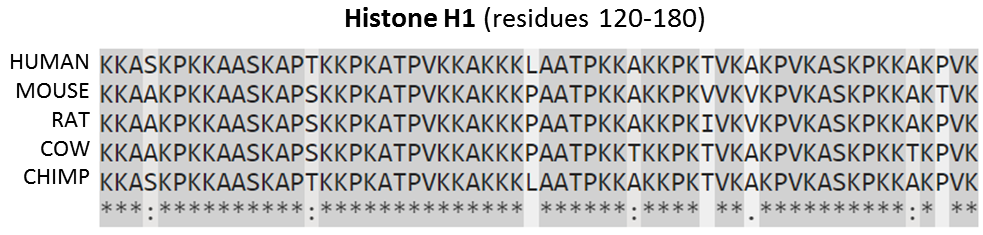
\includegraphics[width=0.8\textwidth]{images/Histone_Alignment.png}
 	\caption{Example of a multiple sequence alignment of amino-acids across biological species.\protect\footnotemark}
	\label{fig:aminoacids}
\end{figure}
\footnotetext{Example from \url{https://en.wikipedia.org/wiki/Sequence_alignment} by T. Shafee.}

This approach can rather straighforwardly be adapted for the multiple alignment of sounds in comparative linguistics. An early example can be seen in Figure~\ref{fig:multialign_bhargava}, aligning various words for `day'. However, one problem with linguistic data is that the assumption of `one element = one letter' is difficult to maintain without strongly simplifying the data. For example, in phonetic transcriptions a single element often consists of multiple Unicode characters, like /aː/ or /t͡ʃ/. In the benchmark data collected by \textcite{list2014benchmark} they opted to put explicit tab marks between the columns, as illustrated by an example from their database in Figure~\ref{fig:multialign_list}.\footnote{The full data is available online at \url{http://alignments.lingpy.org}} A recent development is to allow more columns with different kind of additional information in such files (e.g. data references or expert status). A multialignment then should be just a single column in such a file. Therefor, the column separator for multialignment has become a single space. This is found for example in the data underlying the article by \textcite{hill2017}, an excerpt of which is shown in Table~\ref{tab:data_hill}.\footnote{The full data is available at \url{https://zenodo.org/record/886179}.} This approach is codified in the recent \textit{Cross-Linguistic Data Formats} (CLDF) standard.\footnote{The CLDF specification and documentation is available online at \url{http://cldf.clld.org}.}

\begin{figure}[htbp]
  \centering
  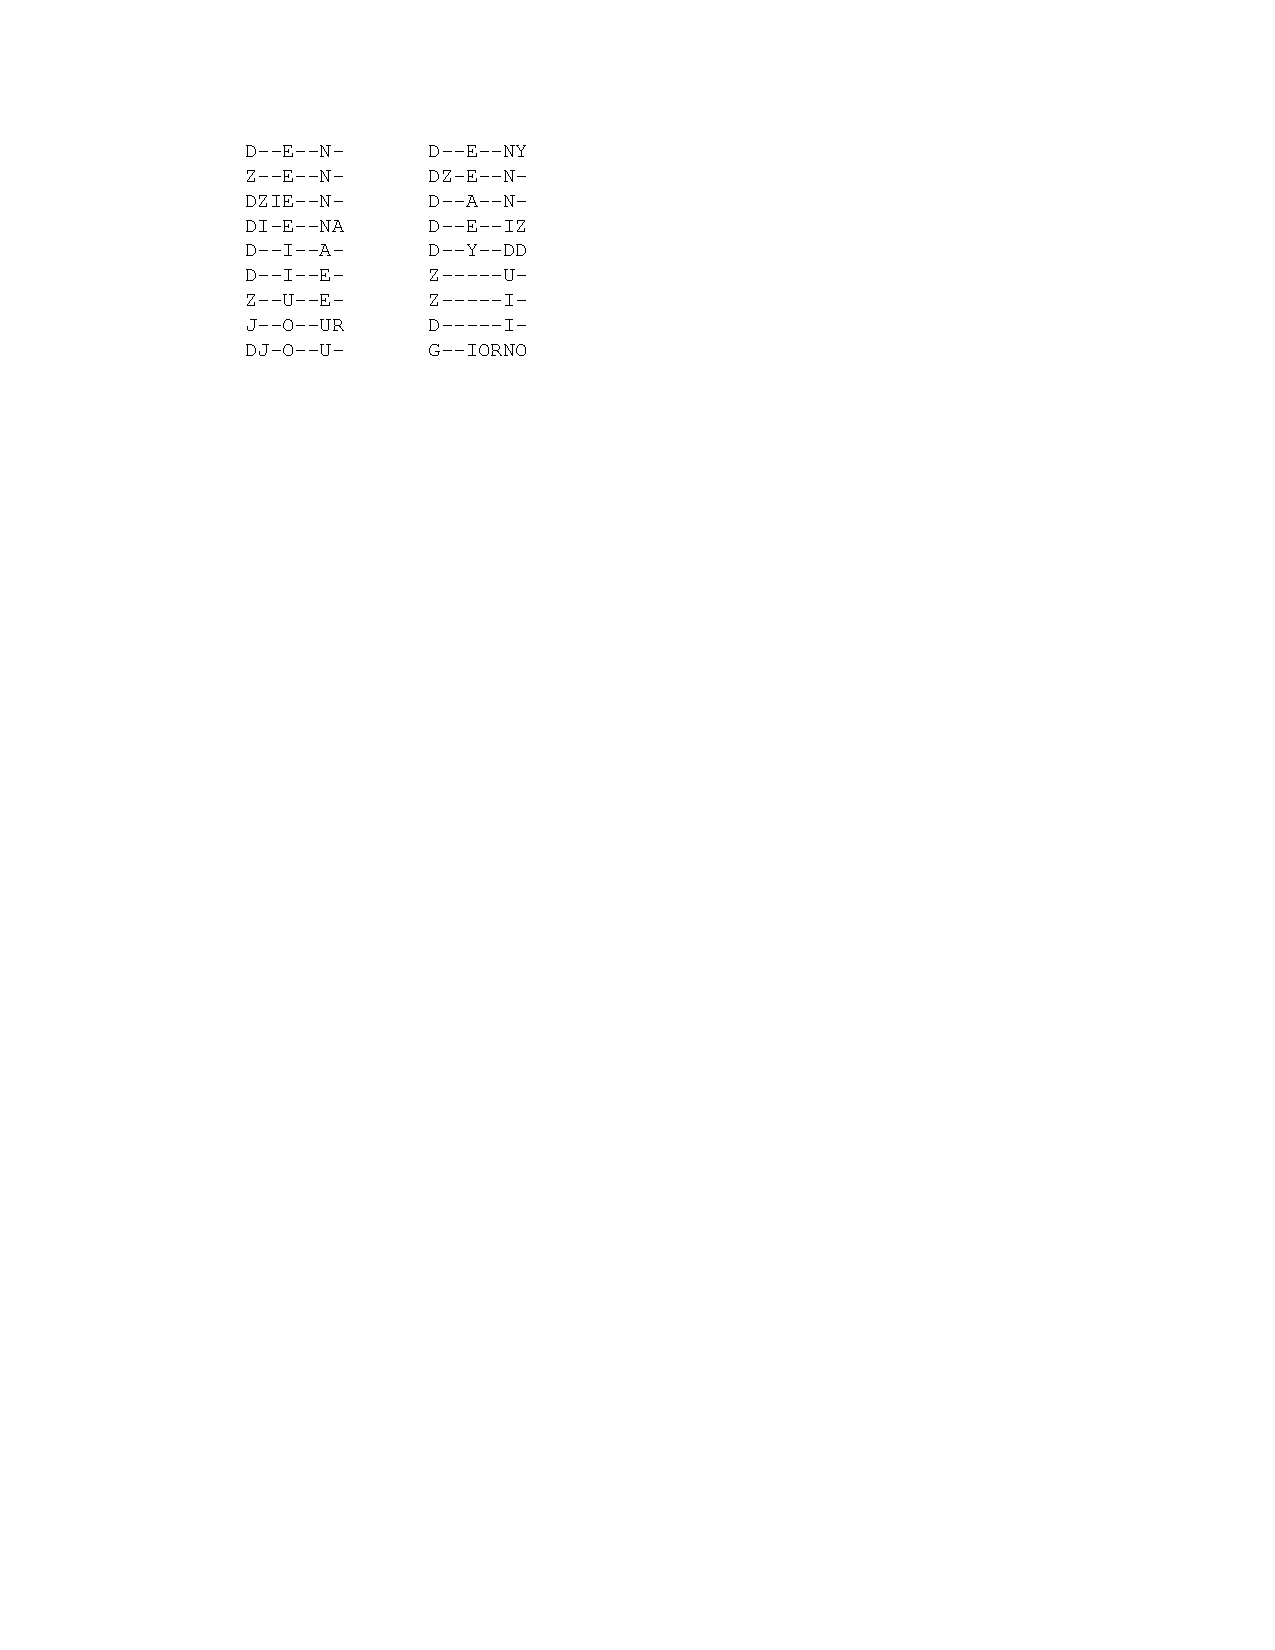
\includegraphics[width=0.5\textwidth]{images/multialign_bhargava.pdf}
  \caption{Linguistic multialignment from \textcite[47]{bhargava2009}.}
  \label{fig:multialign_bhargava}
\end{figure}

\begin{figure}[htbp]
  \centering
  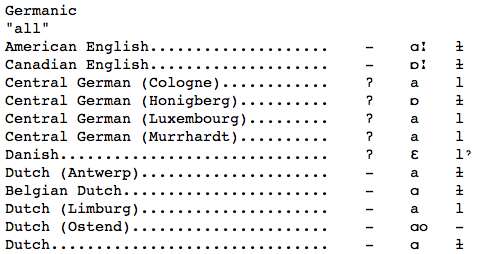
\includegraphics[width=0.8\textwidth]{images/multialign_list.png}
  \caption{Linguistic multialignment with aligned multigraphs and using tabs as separators \parencite{list2014benchmark}.}
  \label{fig:multialign_list}
\end{figure}

\begin{table}[htp]
\centering
\begin{tabular}{llllll}                                              \hline
 ID   & Form        & Cognateset & Alignment           & Source   \\ \hline
 4097 & a³¹tsi³¹    & 501        & a ³¹ + ts i - - ³¹  & Hill2017 \\
 2    & pʐa⁵⁵pʐa⁵⁵  & 33         & p ʐ a ⁵⁵ + p ʐ a ⁵⁵ & Hill2017 \\ 
 5462 & pjɑ̃²²       & 518        & p j ɑ̃ ∼ ²²          & Hill2017 \\ 
 9    & pan³¹ʃɔ̱ʔ⁵⁵  & 567        & p a n ³¹ + ʃ ɔ̰ ʔ ⁵⁵ & Hill2017 \\ 
 10   & pəŋ³¹ʃɔʔ⁵⁵  & 567        & p ə ŋ ³¹ + ʃ ɔ ʔ ⁵⁵ & Hill2017 \\ \hline
\end{tabular}
\caption{Excerpt of data from \textcite{hill2017}}
\label{tab:data_hill}
\end{table}

There are two beta-stage software projects that try to develop a user interface to make it easier to manually edit linguistic multialignment: the Edictor and the MSA-Editor.\footnote{Both project have a common origin. The Edictor is available at \url{https://github.com/digling/edictor}, described in \textcite{list2017}. The MSA-Editor is available at \url{https://github.com/cysouw/msa-editor}.} For the current example we have used the MSA-Editor to prepare the data.

\subsection{Multialignment of words in sentences}

The concept of alignment between languages is also an important notion in the field of machine translation. Parallel translations between languages (or `bitexts' as they are known in computational linguistics, see \cite{tiedemann2011}) are the basic starting point for any machine translation, as this is the principal route to learn equivalent expressions between languages. The classical approach to learn equivalent structure between languages is to align bitexts, i.e. assign a linking between some parts of one sentence (`words') to parts of the translated sentence. The most influential software to perform such bitext alignment has been Giza\texttt{++} \parencite{och2003}. It used a specific output format for aligned sentences, which has become known as the `Pharaoh' format.\footnote{Many names in the statistical machine translation have some kind of reference to Egypt, which seems to be a reference to one of the early highly influential machine translation toolkits, called `EGYPT' \url{http://web.archive.org/web/20060826032742/http://www.clsp.jhu.edu:80/ws99/projects/mt/}.} The Pharaoh-format counts the words, starting at zero, and then links these indices by a dash. For example, the bitext alignment shown in Figure~\ref{fig:bitext_tiedemann} will be summarised in Pharaoh-format as `0-3 1-1 2-1 4-2'.

\begin{figure}[htbp]
  \centering
  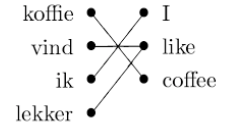
\includegraphics[width=0.4\textwidth]{images/bitext_tiedemann.png}
  \caption{Bitext alignment \parencite[4]{tiedemann2011}.}
  \label{fig:bitext_tiedemann}
\end{figure}

This Pharaoh-format cannot easily be generalized to a multialignment (i.e. for more than two languages). In machine translation there is not much use for alignments with more than two language, so no generalized format has arisen there. For that reason, the Cross-Linguistic Data Formats (CLDF) proposes a special format assigning  abstract cluster-identifiers to each `column' (maybe better called `virtual column', or `functionalEquivalentset' as they are called in the CLDF) in the multialignment.\footnote{See \url{https://github.com/cldf/cldf/blob/master/modules/ParallelText/README.md} for an explanation of the CLDF specification for parallel texts.}

\begin{table}[htp]
\centering
\begin{tabular}{ l c c }            \hline
 Form & Slice & Equivalentset    \\ \hline
 Koffie vind ik lekker & 1 & 1   \\
 Koffie vind ik lekker & 2 & 2   \\
 Koffie vind ik lekker & 3 & 3   \\
 Koffie vind ik lekker & 4 & 4   \\ \hline
 I like coffee         & 1 & 3   \\
 I like coffee         & 2 & 2 4 \\
 I like coffee         & 3 & 1   \\ \hline
 Ich mag gerne Kaffee  & 1 & 3   \\
 Ich mag gerne Kaffee  & 2 & 2   \\
 Ich mag gerne Kaffee  & 3 & 4   \\
 Ich mag gerne Kaffee  & 4 & 1   \\ \hline
\end{tabular}
\caption{Multialignment in the format of the CLDF.}
\label{tab:cldf_paralleltext}
\end{table}

The obvious reason for this format is the crossing lines that occur regularly in word alignment. In sound alignment this also occurs (viz. in metathesis as shown in Figure~\ref{fig:metathesis_list}), but it is not extremely common. For that reason, it is possible to use the `trick' shown in Figure~\ref{fig:metathesis_list}, namely to use two columns for the representation of one alignment.

\begin{figure}[htbp]
  \centering
  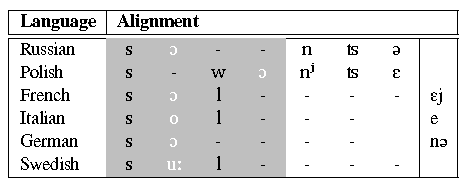
\includegraphics[width=0.8\textwidth]{images/metathesis_list.pdf}
  \caption{Example of multialignment of metathesis \parencite[135]{list2014}.}
  \label{fig:metathesis_list}
\end{figure}

In general this `virtual-column trick' does not work for word alignments within sentences. However, when the languages compared are very similar (like with dialects) then it is possible to use this approach, which is more easily approachable to edit by hand. Therefore, this is the approach that we use for the current project. An excerpt of such an alignement is shown in Table~\ref{tab:wenker_example}.

\begin{table}[htp]
  \centering
  \begin{tabular}{llllllllllll} \hline
    Sie & hat & gesagt & sie & will & es & auch & ihrer & Tochter & es & auch & sagen \\ \hline
	si & hat & gesoat & si & wold & et & oah & hirrer & Doachter & ät & - & soan \\
    sei & - & sot & sei & wollt & et & och & ihrer & Doochte & - & - & sohn \\
    se & - & secht & se & wullt & es & - & ähri & Dochtr & - & ock & säga \\ \hline
  \end{tabular}
  \caption{Multialignment of dialect sentences using `virtual-column trick'}
  \label{tab:wenker_example}
\end{table}

\section{Workflow}

\printbibliography
\end{document}  
